\newprob{mc1}{
    一個物件放在一片凹透鏡前 12 cm 處,產生的成像像距為 8 cm 。若把物
    件移至凹透鏡前 24 cm 處,產生的成像像距為
    % \\    A object is placed 12 cm in front of a concave lens, and the image distance is 8 cm. If the object is moved to a position 24 cm in front of the concave lens, the resulting image distance is
    \begin{tasks}
        \task 6 cm
        \task 12 cm
        \task 16 cm
        \task 18 cm
    \end{tasks}
}{
    \mckey B
}
\newprob{mc2}{
    利用光線箱照亮印有字母``F''的半透明屏 幕。把凸透鏡 $L$ 和屏幕 $S$ 放在適當的距離,以 便在 $S$ 上形成清晰、倒立及等大的成像。下列哪些陳述是正確的?
    % \\A translucent screen printed with a letter ``F'' is illuminated by a ray box. A convex lens $L$ and a screen $S$ are placed so that an inverted sharp image of the same size as the object is produced. Which of the following statements is/are true?
    \bigskip\here{
        \centering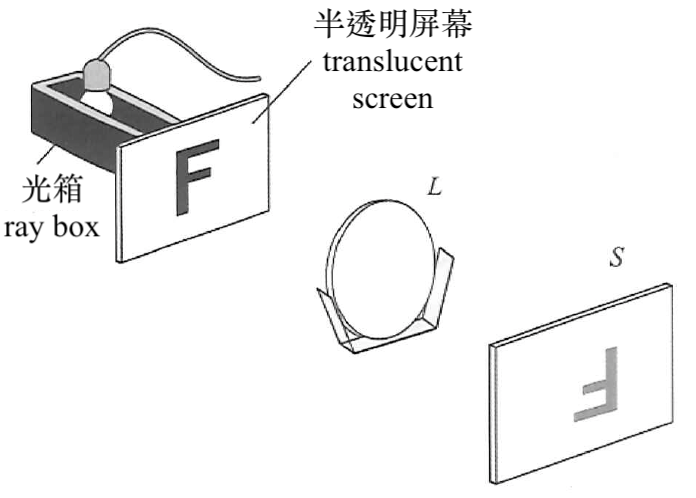
\includegraphics[width=0.35\linewidth]{dedm22n3dnu23.png}
    }\bigskip

    \begin{statements}
        \task 若把 $L$ 略為向右移,成像將向左移。
        % \\        If $L$ is moved to the right through a short distance, the image will move to the left.
        \task 若把 $L$ 略為向上提,成像將向上移。
        % \\
        % If $L$ is raised through a short distance, the image will move upward.
        \task 若把 $L$ 略為向光線箱移動, $S$ 須移離光線 箱,以便再次捕捉成像。
        % \\If $L$ is raised through a short distance, the image will move upward.
    \end{statements}
    \begin{tasks}
        \task 只有(1)
        % \tab\tab (1) only
        \task 只有(1)和(3)
        % \tab\tab (1) and (3) only
        \task 只有(2)和(3)
        % \tab\tab (2) and (3) only
        \task (1), (2) 和 (3)
        % \tab\tab (1), (2) and (3)
    \end{tasks}
}{\mckey C}
\newprob{mc3}{
    如圖顯示,物體藉凸透鏡形成一個倒置的像。 圖中亦繪畫了四條來自這物體的光線。哪條光線是不正確的?
    % \\    An object is placed in front of a convex lens and an inverted image is formed as shown. Four rays from the object are drawn. Which of them is/are incorrectly drawn?
    \bigskip\here{
        \centering
        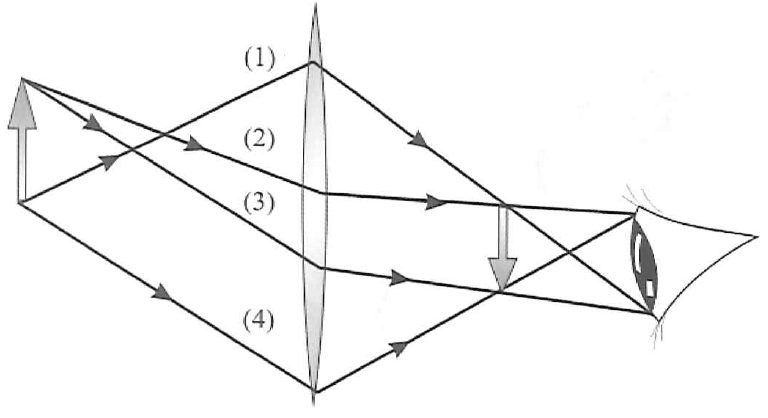
\includegraphics[width=0.35\linewidth]{dedewdwed12dc4f43ge.png}
    }\bigskip

    \begin{tasks}
        \task 只有(1)
        % \tab\tab (1) only
        \task 只有(4)
        % \tab\tab (4) only
        \task 只有(2)和(4)
        % \tab\tab (2) and (4) only
        \task (2), (3) 和 (4)
        % \tab\tab (2), (3) and (4)
    \end{tasks}
}{\mckey C}
\newprob{mc4}{
    如圖顯示,兩條會聚的光線投射在一個主焦點 為 $F$ 的透鏡上。哪字母代表折射線所會聚的 一點?
    % \\    A pair of converging light rays strike a lens with focus $F$ as shown. Which of the letters represents the point where the rays will be converged?
    \bigskip\here{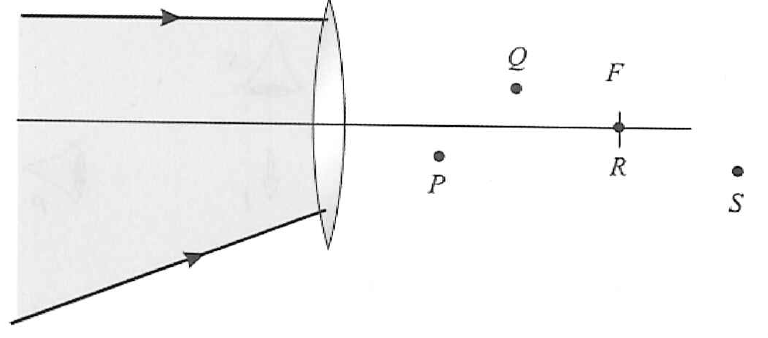
\includegraphics[width=0.4\linewidth]{imdqd9m01u32d-qage.png}}\bigskip
    \begin{tasks}
        \task $P$
        \task $Q$
        \task $R$
        \task $S$
    \end{tasks}
}{\mckey D}
\newprob{mc5}{
    如圖顯示一條光線,穿過凹透鏡 $L$ 後發生的 折射。哪字母可能是 $L$ 的主焦點?
    % \\    A ray of light is refracted by a concave lens $L$ as shown. Which of the letters can be the focus of $L$?
    \bigskip\here{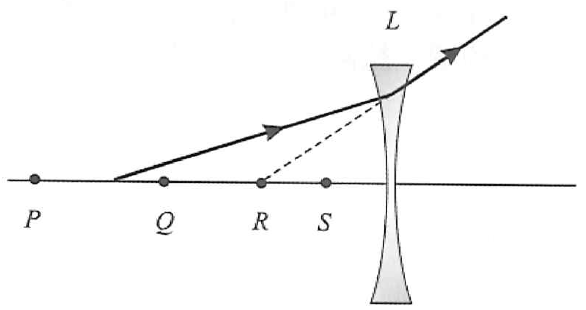
\includegraphics[width=0.45\linewidth]{d8uxdn01ud892.png}}\bigskip
    \begin{tasks}
        \task $P$
        \task $Q$
        \task $R$
        \task $S$
    \end{tasks}
}{\mckey A}
\newprob{mc6}{
    \topalignc{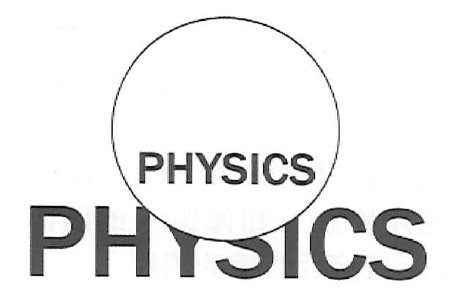
\includegraphics[width=0.4\linewidth]{d2d230dm9i23d9i23932age.png}}\bigskip\\
    如圖顯示,一個透鏡放在印有``PHYSICS'' 字樣的紙板上的情況。以下哪些改變可增加成像的尺寸?
    % \\    The diagram shows the result when a lens is held above a paper printed with the word ``PHYSICS''. Which of the following may increase the size of the image?

    \begin{statements}
        \task 增加透鏡的焦距
        % \\increase the focal length
        \task 把透鏡的位置略為提高
        % \\raise the lens higher
        \task 使用較大折射率的透鏡
        % \\use a lens of larger refractive index
    \end{statements}
    \begin{tasks}
        \task 只有(1)
        \task 只有(1)和(2)
        \task 只有(1)和(3)
        \task 只有(2)和(3)
    \end{tasks}
}{\mckey{A}}

\newprob{mc7}{
    \bigskip\topalignc{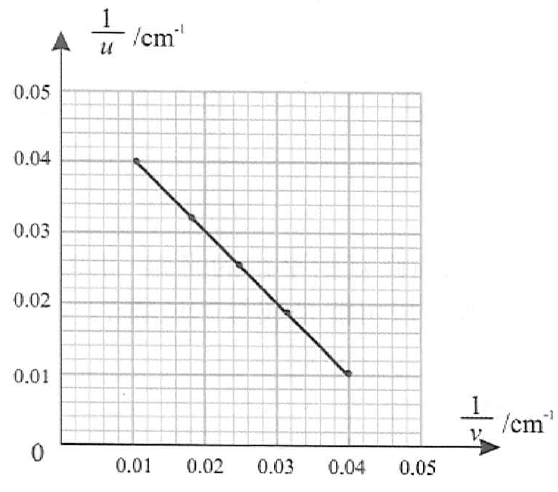
\includegraphics[width=0.5\linewidth]{deudn098u2.png}}\bigskip
    \\把物體放在一個凸透鏡前,並前後移動。然 後記錄物距$v$ 和相應的像距$v$。上圖顯示 $1/u$ 和$1/v$的關係線圖。透鏡的焦距是多少?
    % \\An object is moved in front of a convex lens. The object distance $u$ and the corresponding image distance $v$ are recorded. A graph of $1/u$ against $1/v$ is plotted as shown above. What is the focal length of the lens?
    \begin{tasks}
        \task 10 cm
        \task 15 cm
        \task 20 cm
        \task 25 cm
    \end{tasks}
}{\mckey{C}}
\newprob{mc8}{
    % .\\\par \here{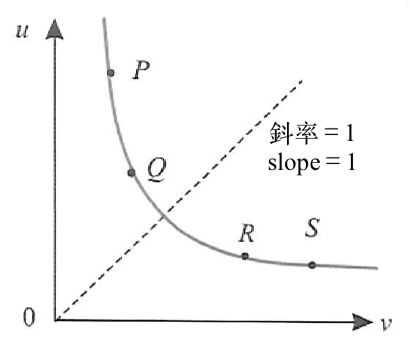
\includegraphics[width=0.35\linewidth]{dijdmioj230.png}}
    \topalignc{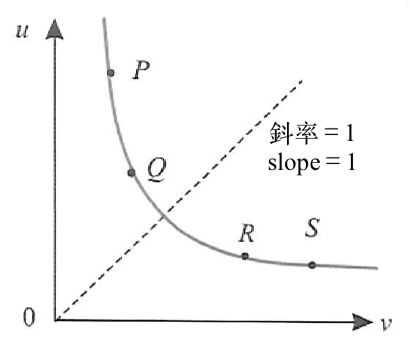
\includegraphics[width=0.35\linewidth]{dijdmioj230.png}}\bigskip
    \\物體沿一個凸透鏡的主軸前後移動。以上的 圖表顯示物距$u$和像距$v$的關係。在哪一點 上,像距最接近透鏡的焦距?
    % \\An object is moved along the principal axis of a convex Lens. The graph above shows a plot of object distance $u$ against image distance $v$. At which of the above points is the image distance most close to the focal length of the lens?
    \begin{tasks}
        \task $P$
        \task $Q$
        \task $R$
        \task $S$
    \end{tasks}

}{\mckey{A}}

\newprob{mc9}{
    一條光線通過兩塊透鏡,並入射線與出射線皆與 主軸平行,如圖。下列哪項正確?
    % A light ray passes two lenses as shown. Both the incident and emergent rays are parallel to the principal axis. Which of the following statements is/are correct?
    \bigskip\here{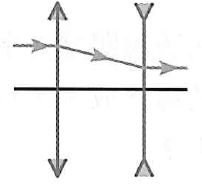
\includegraphics[width=0.2\linewidth]{dqwdqwdun89qdu808n98.png}}\bigskip
    \begin{statements}
        \task 凸透鏡的焦距較凹透鏡長。
        % \\The focal length of the convex lens is longer than that of the concave lens.
        \task 兩塊透鏡各自一個主焦點在凹透鏡右方重 疊。
        % \\One of the foci of the convex lens and one of the foci of the concave lens overlap on the right of the concave lens.
        \task 即使入射線並非平行於主軸,它與出射線仍 然互相平行。
        % \\The incident and the emergent rays are still parallel if the incident ray is not parallel to the principal axis.

    \end{statements}
    \begin{tasks}
        \task 只有(1)
        % \tab\tab (1) only
        \task 只有(3)
        % \tab\tab (3) only
        \task 只有(1)和(2)
        % \tab\tab (1) and (2) only
        \task 只有(2)和(3)
        % \tab\tab (2) and (3) only
    \end{tasks}
}{\mckey C}
\newprob{mc10}{
    把一塊透鏡放在書本前,如圖。
    % \\A lens is placed above a book as shown.
    \bigskip\here{
\includegraphics[width=0.25\linewidth]{dn092i3dn923d32e.png}}\bigskip
    下列哪項正確?
    % \\Which ones are correct?
    \begin{statements}
        \task 透鏡是凹透鏡。\
        % \It is a convex lens.
        \task 成像是虛像。
        % \\ The image is virtual.
        \task 像距較透鏡的焦距短。
        % \\Object distance is shorter than focal length.
    \end{statements}
    \begin{tasks}
        \task 只有(1)和(2)
        % \tab\tab (1) and (2) only
        \task 只有(1)和(3)
        % \tab\tab (1) and (3) only
        \task 只有(2)和(3)
        % \tab\tab (2) and (3) only
        \task (1), (2) 和 (3)
        % \tab\tab (1), (2) and (3)
    \end{tasks}
}{\mckey D}
\newprob{mc11}{
    一個物體通過透鏡成像,如圖。
    % \\An object and its image formed by a lens are as shown.
    \bigskip\here{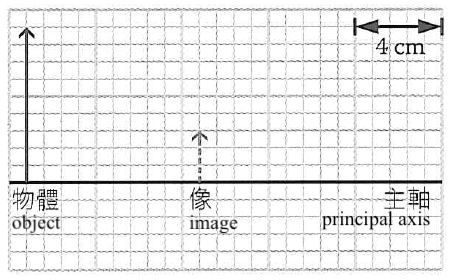
\includegraphics[width=0.5\linewidth]{di0m992imd092-d.png}}\bigskip
    透鏡的焦距是多少?
    % \\What is the focal length of the lens?
    \begin{tasks}
        \task 1 cm
        \task 1.5 cm
        \task 4 cm
        \task 6 cm
    \end{tasks}
}{\mckey D}

\newprob{mc13}{
    一束會聚光線射向凹透鏡,並在距離透鏡10 cm 外的 P 點會聚。已知透鏡焦距為4 cm。若移開 透鏡,光線會在 Q 點會聚。
    % \\    A convergent beam is incident on a concave lens of focal length 4 cm as shown. It converges at P, which is 10 cm from the lens. If the lens is taken away, the beam will converge at Q.
    \bigskip\here{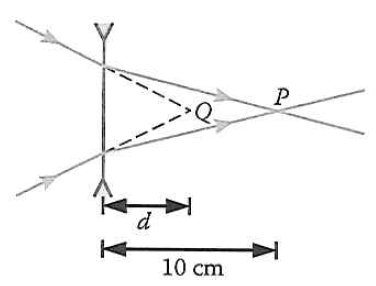
\includegraphics[width=0.25\linewidth]{d9nd8u92309823.png}}\bigskip
    Q點距離透鏡多遠?
    % \\How far is Q from the position of the lens?
    \begin{tasks}
        \task 2.5 cm
        \task 2.9 cm
        \task 4 cm
        \task 6.7 cm
    \end{tasks}
}{\mckey B}
\newprob{mc14}{
    下圖顯示某個像的線性 放大率 $m$ 隨像距$v$ 的 變化。
    % \\The graph shows how the linear magnification $m$ of an image varies with its distance from the lens $v$.
    \bigskip\here{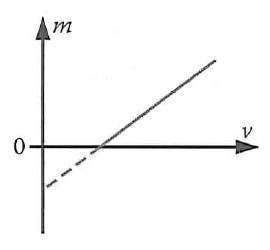
\includegraphics[width=0.25\linewidth]{du8nu903d2.png}}\bigskip
    今使用另一塊焦距較長的透鏡。下列哪幅線圖正 確?(原有線圖以短虛線表示。)
    % \\   A lens of a longer focal length is used instead. Which of the following graphs is correct? (The original graph is shown by the dotted line.)
    \begin{tasks}
        (2)
        \task
        \topalign{\includegraphics[width=0.55\linewidth]{ddqwð3dun3298dge.png}}
        \task
        \topalign{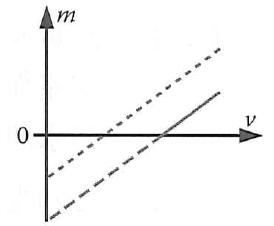
\includegraphics[width=0.55\linewidth]{dn0892ud023.png}}
        \task
        \topalign{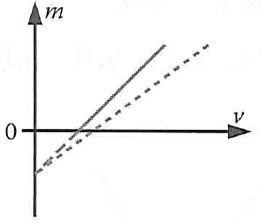
\includegraphics[width=0.55\linewidth]{dnu98ud298dun923d.png}}
        \task
        \topalign{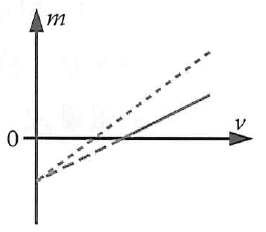
\includegraphics[width=0.55\linewidth]{dud2u0n2ndu8dge.png}}
    \end{tasks}

}{\mckey D}
\newprob{mc15}{
    現有一個固定的發光物件和一個固定的屏幕,物件和屏幕間的距離為 5 m。當一片焦距為 1.3 m 的透鏡放在物件前
    $x$ m 時,以下哪項是$x$ 的可能值?
    % \\    There is a fixed luminous object and a fixed screen, with a distance of 5 m between them. When a lens with a focal length of 1.3 m is placed at a distance of $x$ m in front of the object, which of the following is a possible value for $x$?
    \begin{tasks}
        \task $1.12$
        \task $1.88$
        \task $2.60$
        \task $x$ 無解
    \end{tasks}
}{\mckey D}

\newprob{mc12}{
    把一根蠟燭放在牆壁前一段距離外。在兩者之間 放置一塊透鏡,並緩慢移動透鏡。當透鏡移至途 中兩點,均有清晰的像在牆壁上形成。蠟燭在兩 處的像高分別為50 cm 和8 cm。問蠟燭的高度 是多少?
    % \\    A candle is placed at a fixed distance in front of a wall. A lens is inserted and moved slowly between them. At two Particular positions, sharp images are formed on the wall. The heights of the images are 50 cm and 8 cm respectively. What is the height of the candle?
    \begin{tasks}
        \task 6.25 cm
        \task 20 cm
        \task 21 cm
        \task 29 cm
    \end{tasks}
}{\mckey B}

% \newprob{mc16}{
%     現有一個固定的發光物件和一個固定的屏幕。當一片透鏡分別放在物件前
%     1 m 和 4 m 時,屏幕上出現了高度分別為 $h_1$ 和 $h_2$ 的成像。求 $h_1$: $h_2$。
%     % \\        There is a fixed luminous object and a fixed screen. When a lens is placed at distances of 1 m and 4 m in front of the object respectively, two images with heights of $h_1$ and $h_2$ appear on the screen. The task is to find the ratio $h_1:h_2$.
%     \begin{tasks}
%         \task $16:1$
%         \task $4:1$
%         \task $2:1$
%         \task $1:2$
%     \end{tasks}
% }{B}